\documentclass{beamer}

\usepackage[utf8]{inputenc}
\usepackage[spanish]{babel}
\usepackage[outputdir=.build]{minted}
\usepackage{hyperref}
\usepackage{graphicx}

\hypersetup{
    colorlinks = true
}

\usetheme{Madrid}

%Information to be included in the title page:
\title{Taller de Física Computacional}
\subtitle{Bucles}
\author{Cristián G. Sánchez y Carlos J. Ruestes}
\date{2020}

\begin{document}

\frame{\titlepage}

%%%%%%%%%%%%%%%%%%%%%%%%%%%%%%%%%%%%%%%%%%%%%%%%%%%%%%%%%%
\begin{frame}[fragile]
    \frametitle{Bucles}
    \begin{block}{Bucle}
        El bucle es una estructura que nos permite ejecutar en forma repetida un conjunto de declaraciones.
        \begin{itemize}
            \item La repetición puede ser infinita o finita.
            \item La terminación de la repetición se hace en base a una expresión lógica.
            \item Se puede \alert{escapar} de una repetición.
        \end{itemize}
    Con los bucles y condicionales (sobre lo que ya vimos) en principio podemos programar lo que querramos.
    \end{block}
\end{frame}

%%%%%%%%%%%%%%%%%%%%%%%%%%%%%%%%%%%%%%%%%%%%%%%%%%%%%%%%%%

\begin{frame}[fragile]
    \frametitle{La declaración de bucle más completa}

\begin{columns}
    \begin{column}{0.5\textwidth}
        \begin{minted}[showspaces=true,autogobble=true]{python}
        while (condición):
            # Bloque 1
            # esto se repite mientras
            # la condición sea True
        else:
            # Bloque 2
            # esto se ejecuta 
            # por única vez
            # si la condición es False
            # y es opcional
        \end{minted}
    \end{column}
    \begin{column}{0.5\textwidth}
        \begin{center}
            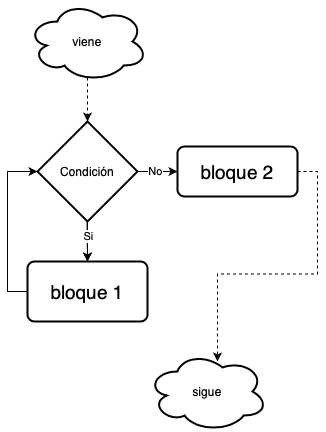
\includegraphics[height=7cm]{figuras/flow_while.png}           
        \end{center}    
    \end{column}

\end{columns}
 \end{frame}

%%%%%%%%%%%%%%%%%%%%%%%%%%%%%%%%%%%%%%%%%%%%%%%%%%%%%%%%%%
\begin{frame}[fragile]
    \frametitle{Escape del bucle}
    \begin{block}{Bucle}
        Dentro del bloque que sigue al \mintinline{python}{while} pueden utilizarse las siguientes palabras clave para alterar el flujo:
        \begin{itemize}
            \item La invocación de la palabra clave \mintinline{python}{break} sale incondicionalmente del bucle sin ejecutar el bloque que sigue
            al \mintinline{python}{else} (si existiera).
            \item La invocación de la palabra clave \mintinline{python}{continue} saltea el resto del bloque y vuelve a la evaluación de la condición
            presente en el \mintinline{python}{while}.
        \end{itemize}
    \end{block}
    Las palabras clave \mintinline{python}{break} y \mintinline{python}{continue} suelen ser parte de declaraciones condicionales que 
    permiten terminar o proseguir el bucle en base a otras condiciones.
\end{frame}

%%%%%%%%%%%%%%%%%%%%%%%%%%%%%%%%%%%%%%%%%%%%%%%%%%%%%%%%%%
\begin{frame}[fragile]
    \frametitle{Bucle infinito}
    \begin{block}{Bucle infinito}
    \begin{minted}[showspaces=true,autogobble=true]{python}
        while True:
            # esto se repite hasta
            # que el programa se interrumpa
    \end{minted}
    \end{block}
    La combinación con una (o más) invocaciones a \mintinline{python}{break} dentro de una declaración condicional permite
    hacer cualquier bucle de esta manera.
\end{frame}

%%%%%%%%%%%%%%%%%%%%%%%%%%%%%%%%%%%%%%%%%%%%%%%%%%%%%%%%%%
\begin{frame}[fragile]
    \frametitle{Iteración sobre una serie de naturales consecutivos}
    \begin{block}{Bucle sobre $n\in\mathbb{N}$}
    Podemos construir un bulce sobre una serie de enteros consecutivos de la siguiente forma:
    \begin{minted}[showspaces=true,autogobble=true]{python}
        i = 0 # se parte de i = 0
        while (i <= maxn):
            # esto se repite hasta que i == nmax
            #
            i += 1 # aquí se incrementa i
    \end{minted}
    \end{block}
\end{frame}

%%%%%%%%%%%%%%%%%%%%%%%%%%%%%%%%%%%%%%%%%%%%%%%%%%%%%%%%%%
\begin{frame}[fragile]
    \frametitle{Bucles anidados}
    \begin{block}{Bucles anidados}
    Podemos anidar bucles dentro de bucles para llevar a cabo iteraciones sobre conjuntos más complejos:
    \begin{minted}[showspaces=true,autogobble=true]{python}
        i = j = k = 0 # se parte de i,j,k = 0
         while (i <= maxi):
            while (j <= maxj):
                while (k <= maxk):
                    # esto se repite hasta que  
                    # (i == maxi) and (j == maxj) and (k == maxk)
                    k += 1 # aquí se incrementa k
                j += 1 # aquí se incrementa j
            i += 1 # aquí se incrementa i
    \end{minted}
    \end{block}
\end{frame}

%%%%%%%%%%%%%%%%%%%%%%%%%%%%%%%%%%%%%%%%%%%%%%%%%%%%%%%%%%

\begin{frame}[fragile]
    \frametitle{Bucles y eficiencia}

\begin{columns}
    \begin{column}{0.3\textwidth}
        
\includegraphics[width=3cm]{figuras/sin.png}
    \end{column}
    \begin{column}{0.7\textwidth}
        Los bucles anidados son ingredientes fundamentales de cualquier programa. Muchas operaciones comunes en física computacional,
        desde las multiplicaciones matriciales, contracciones tensoriales, transformadas de Fourier o la simple evaluación de una función 
        de varias variables en una grilla requieren de bucles anidados para ejecutarse. Los bucles en Python son {\em lentos}. Frustrantemente
        lentos de hecho, en algunos casos. Hasta el punto de volver las operaciones antes mencionadas prácticamente imposibles salvo
        para casos triviales. Esta es una de las razones de la existencia del paquete NumPy que permite llevar a cabo \alert{algunos}
        bulces utilizando lo que se denomina {\em vectorización} llamando a rutinas específicas en {\tt C} para cada caso.
    \end{column}

\end{columns}
 \end{frame}

%%%%%%%%%%%%%%%%%%%%%%%%%%%%%%%%%%%%%%%%%%%%%%%%%%%%%%%%%%%
\begin{frame}
\frametitle{Síntesis y recursos:}

\begin{itemize}
\item \href{https://es.wikipedia.org/wiki/Bucle_while}{Bucle while en Wikipedia en español}
\item \href{https://en.wikipedia.org/wiki/While_loop}{Bucle while en Wikipedia en ingles}

\end{itemize}
\end{frame}

\end{document}
